\documentclass[aspectratio=169,10pt]{beamer}
\usetheme{Madrid}
\usecolortheme{seahorse}
\usepackage{booktabs}
\usepackage{graphicx}
\usepackage{listings}
\usepackage{tikz}
\usetikzlibrary{shapes.geometric, arrows.meta, positioning}
\graphicspath{{../figures/}}

\lstset{
  basicstyle=\ttfamily\scriptsize,
  breaklines=true,
  backgroundcolor=\color{gray!10},
}

\title{bn-en-translate}
\subtitle{Local GPU-Accelerated Bengali-to-English NMT\\
with LoRA Fine-Tuning and Hardware-Aware Deployment}
\author{Souradeepta Biswas}
\institute{M.S. Computer Science, Syracuse University \\ Independent Researcher}
\date{2026}

\begin{document}

\begin{frame}
  \titlepage
\end{frame}

\begin{frame}{Table of Contents}
  \tableofcontents
\end{frame}

% ── Motivation ──────────────────────────────────────────────────────────────
\section{Motivation}

\begin{frame}{Why Bengali NMT on Consumer Hardware?}
  \begin{columns}
    \column{0.55\textwidth}
    \begin{itemize}
      \item Bengali: \textbf{234 million} native speakers --- 6th most spoken language
      \item NLP tooling severely underdeveloped relative to speaker population
      \item Existing solutions require cloud APIs: privacy risk, latency, cost
      \item Rich literary tradition (Tagore, Nazrul) --- high demand for quality translation
      \item \textbf{Goal:} fully offline, GPU-accelerated Bengali $\to$ English on a \$700 laptop
    \end{itemize}
    \column{0.4\textwidth}
    \begin{block}{Hardware Target}
      NVIDIA RTX 5050 (sm\_120)\\
      Blackwell, 8\,GB GDDR7\\
      AMD Ryzen 5 240 (Zen 4)\\
      16\,GB RAM, WSL2 Ubuntu
    \end{block}
    \vspace{0.3cm}
    \begin{alertblock}{No API keys required}
      Fully open-source stack
    \end{alertblock}
  \end{columns}
\end{frame}

% ── Architecture ─────────────────────────────────────────────────────────────
\section{System Architecture}

\begin{frame}{Four-Stage Translation Pipeline}
  \begin{center}
  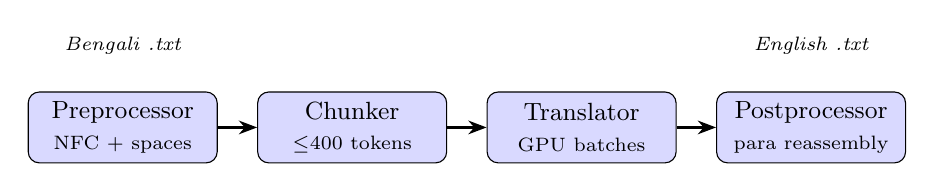
\begin{tikzpicture}[
    box/.style={rectangle, rounded corners, draw, fill=blue!15,
                minimum width=2.4cm, minimum height=0.9cm, font=\small, align=center},
    arrow/.style={-{Stealth}, thick},
    node distance=0.7cm and 0.5cm
  ]
    \node[box] (pre)   {Preprocessor\\\scriptsize NFC + spaces};
    \node[box, right=of pre]   (chunk) {Chunker\\\scriptsize $\le$400 tokens};
    \node[box, right=of chunk] (trans) {Translator\\\scriptsize GPU batches};
    \node[box, right=of trans] (post)  {Postprocessor\\\scriptsize para reassembly};

    \draw[arrow] (pre) -- (chunk);
    \draw[arrow] (chunk) -- (trans);
    \draw[arrow] (trans) -- (post);

    \node[above=0.35cm of pre,  font=\scriptsize\itshape] {Bengali .txt};
    \node[above=0.35cm of post, font=\scriptsize\itshape] {English .txt};
  \end{tikzpicture}
  \end{center}

  \begin{columns}
    \column{0.48\textwidth}
    \begin{itemize}
      \item Chunker never splits mid-sentence
      \item Danda \texttt{।}/\texttt{॥} aware sentence boundaries
      \item \texttt{para\_id} metadata drives reassembly
    \end{itemize}
    \column{0.48\textwidth}
    \begin{itemize}
      \item Same paragraph count guaranteed in/out
      \item Optional Ollama literary polish pass
      \item CTranslate2 float16 or HF native backends
    \end{itemize}
  \end{columns}
\end{frame}

% ── Models ────────────────────────────────────────────────────────────────────
\section{Models}

\begin{frame}{Evaluated Models}
  \begin{table}
  \small
  \begin{tabular}{llrrrl}
    \toprule
    Key & Architecture & VRAM & FLORES BLEU & chrF & Backend \\
    \midrule
    \texttt{nllb-600M}       & M2M-100   & 2.0\,GB & \textbf{55.3} & \textbf{72.8} & CT2 float16 \\
    \texttt{seamless-medium} & Custom    & 3.9\,GB & \textbf{67.0} & \textbf{80.2} & HF float16  \\
    \texttt{nllb-1.3B}       & M2M-100   & 2.6\,GB & $\sim$26 (lit.) & --- & CT2 float16 \\
    \texttt{indicTrans2-1B}  & M2M-100v  & 3.0\,GB & $\sim$44 (lit.) & --- & CT2 float16 \\
    \midrule
    \texttt{madlad-3b}       & T5        & 8.1\,GB & \multicolumn{2}{c}{\textit{excluded$^\dagger$}} & HF float16  \\
    \bottomrule
  \end{tabular}
  \end{table}
  \vspace{0.1cm}
  \footnotesize $^\dagger$ Checkpoint weight mismatch + VRAM constraint (8\,GB insufficient for 3B float16).\\
  Bold values = directly measured on FLORES-200 devtest (90 sentences).
\end{frame}

% ── Results ───────────────────────────────────────────────────────────────────
\section{Results}

\begin{frame}{Benchmark Results --- FLORES-200 Devtest (90 sentences)}
  \begin{columns}
    \column{0.48\textwidth}
    \begin{block}{NLLB-600M CT2 float16}
      BLEU \textbf{55.3} / chrF \textbf{72.8}\\
      Throughput: \textbf{197\,chars/s}\\
      VRAM: 2,056\,MiB\\
      Time per sentence: 0.10\,s
    \end{block}
    \vspace{0.25cm}
    \begin{block}{Seamless-v2-large HF float16}
      BLEU \textbf{67.0} / chrF \textbf{80.2}\\
      Throughput: \textbf{32\,chars/s}\\
      VRAM: 3,919\,MiB\\
      Time per sentence: 1.33\,s
    \end{block}

    \column{0.48\textwidth}
    \begin{alertblock}{Trade-off}
      Seamless: +11.7 BLEU (+21\%)\\
      but $6\times$ more VRAM and\\
      $13\times$ slower throughput.\\
      \vspace{0.15cm}
      Choose by use-case:\\
      real-time $\to$ NLLB\\
      best quality $\to$ Seamless
    \end{alertblock}
    \vspace{0.2cm}
    \begin{block}{LoRA Fine-tuning}
      3 epochs, 7,863 pairs, bf16\\
      eval\_loss: $2.111 \to 1.992$\\
      Runtime: 2.46\,h on RTX 5050
    \end{block}
  \end{columns}
\end{frame}

\begin{frame}{Per-Domain BLEU (NLLB-600M, Custom 90-Sentence Corpus)}
  \begin{center}
    
\includegraphics[width=0.75\textwidth]{domain_bleu.png}
  \end{center}
  \vspace{-0.1cm}
  \small Single-number BLEU masks a \textbf{75-point domain spread} (News: 4.7 $\leftrightarrow$ Health: 80.6).
\end{frame}

\begin{frame}{Model Comparison}
  \begin{center}
    
\includegraphics[width=0.85\textwidth]{combined_results.png}
  \end{center}
\end{frame}

% ── Hardware Constraints ─────────────────────────────────────────────────────
\section{Hardware Constraints}

\begin{frame}{Six Blackwell sm\_120 Deployment Constraints}
  \begin{enumerate}
    \item \textbf{CTranslate2 INT8 fails} --- \texttt{CUBLAS\_STATUS\_NOT\_SUPPORTED} on sm\_120+CUDA 12.x;
          use float16 with a real-translation probe at load time
    \item \textbf{Tokenizer fork deadlock} --- HuggingFace fast tokenizer + forked DataLoader workers;
          fix: \texttt{TOKENIZERS\_PARALLELISM=false}
    \item \textbf{bf16 required for training} --- fp16 GradScaler raises \texttt{ValueError};
          \texttt{bf16=True} bypasses GradScaler; Blackwell supports bf16 natively
    \item \textbf{SeamlessM4T device\_map} --- \texttt{device\_map="auto"} unsupported;
          must use \texttt{.to("cuda")} after float16 load
    \item \textbf{MADLAD embedding tie} --- local checkpoint has mismatched \texttt{shared.weight};
          produces degenerate output silently; re-download or use cloud
    \item \textbf{CT2 batch OOM} --- 900+ sentences at once $\to$ CUDA OOM;
          fix: \texttt{max\_batch\_size=32}
  \end{enumerate}
  \vspace{0.2cm}
  All constraints root-caused, fixed, and regression-tested in 212 unit/integration tests.
\end{frame}

% ── Conclusion ───────────────────────────────────────────────────────────────
\section{Conclusion}

\begin{frame}{Conclusion}
  \begin{itemize}
    \item \textbf{bn-en-translate}: fully offline Bengali$\to$English NMT on a consumer GPU
    \item NLLB-600M: \textbf{55.3 BLEU / 72.8 chrF} at 197\,ch/s on 2\,GB VRAM
    \item Seamless-v2: \textbf{67.0 BLEU / 80.2 chrF} at 3.9\,GB VRAM --- best consumer-GPU result
    \item LoRA fine-tuning fully unlocked on Blackwell sm\_120 with bf16
    \item Six previously undocumented hardware constraints documented and resolved
    \item 212 TDD tests, run in 27\,s
  \end{itemize}
  \vspace{0.4cm}
  \begin{center}
    \large\textbf{github.com/souradeepta/translate}
  \end{center}
\end{frame}

\end{document}
